\documentclass[a4paper,twoside]{report}
\usepackage[utf8]{inputenc}
% \usepackage[a4paper, width=150mm, top=25mm, bottom=25mm, bindingoffset=6mm]{geometry}
\usepackage{fancyhdr}
\pagestyle{fancy}
 \fancyhead{}
 \fancyhead[LO,LE]{\leftmark}
 \fancyfoot{}
 \fancyfoot[CO,CE]{\thepage}
 \renewcommand{\headrulewidth}{0.2pt}
 \renewcommand{\footrulewidth}{0.2pt}
 \setlength{\headheight}{14.5pt}


% \usepackage{epsfig,epic,eepic,units}
\usepackage{hyperref} %allows to add hyperlinks and cross reference in-text
\usepackage{textcomp} %this is for symbols such as copyright etc
\usepackage{url} %for adding urls obvs so they appear always in one line without breaks
\usepackage{longtable} %allows you to make tables of two or more pages
\usepackage{mathrsfs} %maths fonts, might not need
\usepackage{array} %extends array and tabular environments
\usepackage{multirow} %for tables again
\usepackage{bigstrut} %tables
\usepackage{amssymb} %adding arrows tbh for chemistry you can just use chemmacros \begin{reaction} environment
\usepackage{amsmath} %for writing maths
\usepackage{adjustbox}%supplement to graphics package
\usepackage{graphicx}
\usepackage{lscape} %allows to add certain pages in landscape
\usepackage[nottoc]{tocbibind} %this adds bibliography to your ToC
\usepackage{textgreek} %for upright greek letters
\usepackage{siunitx} %you can declare the units you want as necessary read documentation
\usepackage{biblatex}
\usepackage[
    asymmetric,
    a4paper,
    left=3cm,
    right=2cm,
    top=2.75cm,
    bottom=3cm,
    footskip=20pt,
    twoside]{geometry}

    \usepackage{tikz}
\usetikzlibrary {automata, positioning, shapes, arrows.meta}
\usepackage{enumitem}
\usepackage{pifont}

% add commands
\usepackage{commands}


\addbibresource{refs.bib}

\begin{document}
\sloppy

\section{Block graph}

\begin{figure}[ht]
  \centering
  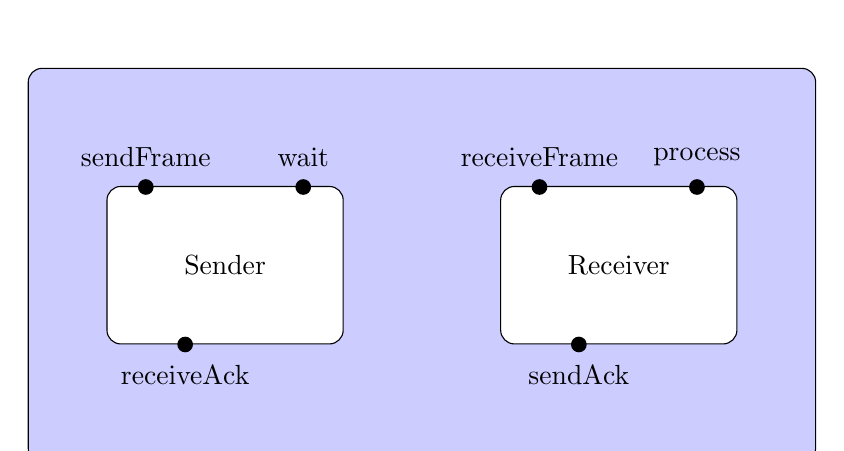
\begin{tikzpicture}
    % Outer blue rectangle with text
    \node[draw, fill=blue!20, rounded corners=5pt, minimum width=10cm, minimum height=5cm, anchor=south west]
    (Main) at (0,0) {};

    \node[draw, fill=white, rounded corners=5pt, minimum width=3cm, minimum height=2cm, anchor=south west, align=left]
    (Sender) at (1,1.5) {Sender};

    \node[circle, fill=black, inner sep=2pt] (sendFrameBase) at (1.5,3.5) {};
    \node[above=1pt of sendFrameBase] (sendFrame) {sendFrame};

    \node[circle, fill=black, inner sep=2pt] (waitBase) at (3.5,3.5) {};
    \node[above=1pt of waitBase] (wait) {wait};

    \node[circle, fill=black, inner sep=2pt] (receiveAckBase) at (2,1.5) {};
    \node[below=1pt of receiveAckBase] (receiveAck) {receiveAck};

    \node[draw, fill=white, rounded corners=5pt, minimum width=3cm, minimum height=2cm, anchor=south west, align=left]
    (Receiver) at (6,1.5) {Receiver};

    \node[circle, fill=black, inner sep=2pt] (receiveFrameBase) at (6.5,3.5) {};
    \node[above=1pt of receiveFrameBase] (receiveFrame) {receiveFrame};
    \node[circle, fill=black, inner sep=2pt] (processBase) at (8.5,3.5) {};
    \node[above=1pt of processBase] (process) {process};
    \node[circle, fill=black, inner sep=2pt] (sendAckBase) at (7,1.5) {};
    \node[below=1pt of sendAckBase] (sendAck) {sendAck};


  \end{tikzpicture}
\end{figure}


% \printbibliography

\end{document}
